The recommender system is setup as a scalable web application. Divided as follows.

\subsection{Scrapers}
\label{sec:arch:scrapers} 
Our back-end consists of scraper application that collect data from different websites, extract movie mentions and store these in \textbf{MondoDB}.  

\subsection{Neo4j}
\label{sec:arch:neo4j}
This a distributed graph database. Extracted mentions are then imported into \textbf{Neo4j}. 

\subsection{GraphSearch}
\label{sec:arch:graphsearch}
Input from the front-end web application is parsed and then converted to a Neo4j compatible query. The response is then returned to the web application.

\subsection{Web application}
\label{sec:arch:webapplication}

NGINX, Passenger, Sinatra

\begin{figure}[H]
	\centering
	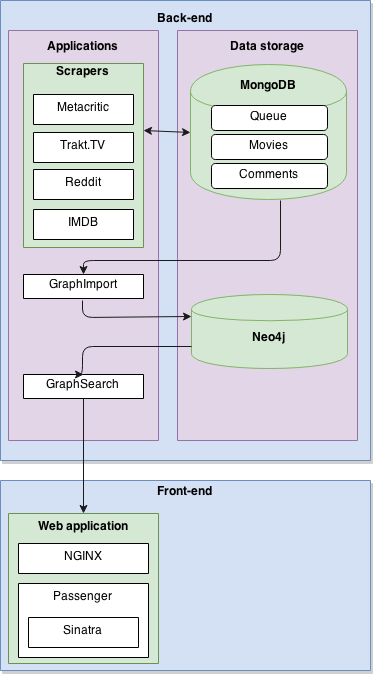
\includegraphics[width=\linewidth]{pipeline.png}
	\caption{Pipeline}
\end{figure}

\subsection{Scalability}
\label{sec:arch:scalability} 
More on the scalability of our scripts, mongoDB, Neo4j and the front-end webserver.